\documentclass[a4paper, 12pt]{article}
\usepackage{graphicx}
\usepackage{enumitem}
\usepackage{mathtools}
\usepackage{hyperref}
\usepackage{caption}
\usepackage{subcaption}
\def\code#1{\texttt{#1}}
\def\f#1{Figure \ref{fig:#1}}
\begin{document}

\title{\vspace{4.0cm}Applied GPU Programming - Assignment IV\\
\large DD2360 HT20}
\author{Pontus Asp}
\date{\today}
\maketitle
\thispagestyle{empty}
\pagenumbering{roman}
\newpage

\clearpage
\pagenumbering{arabic}

% Write here ->
\section{Git repository}
I uploaded my git repository to GitHub. I use the same git repository for the entire course but the folder structure requested is still followed under the root folder. I also have 2 extra directories, one for this report and one where I have code from lectures. I also was not sure if Exercise 4 should have been separate or included in this report so I did both, the standalone Exercise\_4.pdf can be found under the ex\_4 folder.
\\\\
Here is the link to my git repository:\\
\url{https://github.com/pontusasp/kth-dd2360/tree/master/Assignment_4}

% List and explain your extensions to the basic template provided by the course.
\section{Exercise 1}

% Explain how you solved the issue when the ARRAY_SIZE is not a multiple of the block size. If you implemented timing in the code, vary ARRAY_SIZE from small to large, and explain how the execution time changes between GPU and CPU.
\section{Exercise 2}

% 1. Measure the execution time of the CPU version, varying the number of particles.
%
% 2. Measure the execution time of the GPU version, varying the number of particles, like in 1).
%   2.1. Include data copying time to and from in the measurement.
%   2.2. For each GPU particle configuration, vary the block size in the GPU version from 16, 32, …, up to 256 threads per block.
%
% 3. Generate one or more performance figures based on your measurements in 1 and 2. Include it in the report with a description of the experimental setup (e.g., GPU used) and the observations obtained from the results. Explain how the execution time of the two version changes when the number of particles increases. Which block size configuration is optimal?
%
% 4. Currently, the particle mover is completely offloaded to the GPU, only with data transfer at the beginning and end of the simulation. If the simulation involves CPU dependent functions (i.e. particles need to be copied back and forth every time step), would your observation in 3) still holds? How would you expect the performance will change in terms of GPU execution? Make an educated guess by timing your kernels.
%
% Important note: If the execution times between the CPU and the GPU are very similar, try to increase the number of particles and the number of iterations per simulation even further.
%
\section{Bonus Exercise}


% WRITE STANDALONE FILE FIRST
\section{Exercise 4}
% WRITE STANDALONE FILE FIRST

% Write here <--

\end{document}



%\begin{figure}
%  \centering
%  \begin{subfigure}{.5\textwidth}
%    \centering
%    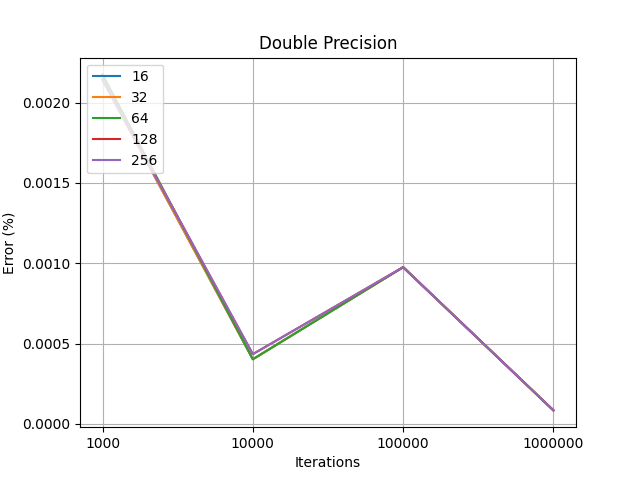
\includegraphics[width=1\linewidth]{graphs/ex_bonus_double_error.png}
%    \caption{Double Precision}
%    \label{fig:ex-single-double-error}
%  \end{subfigure}%
%  \begin{subfigure}{.5\textwidth}
%    \centering
%    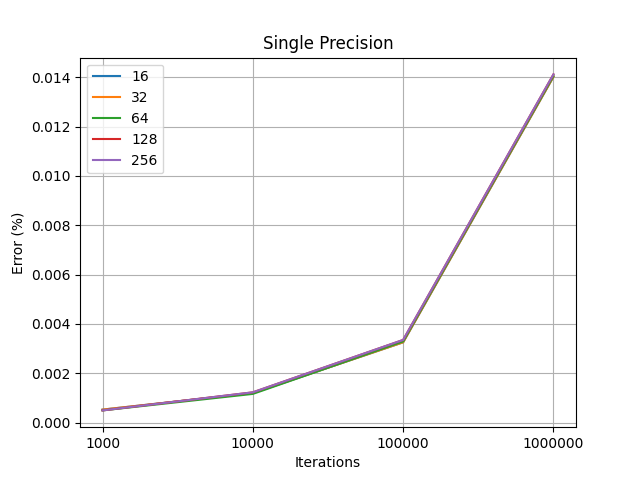
\includegraphics[width=1\linewidth]{graphs/ex_bonus_single_error.png}
%    \caption{Single Precision}
%    \label{fig:ex-bonus-single-error}
%  \end{subfigure}
%  \caption{Graphs of error using double and single precision with different amounts of iterations and block sizes.}
%  \label{fig:fig:ex-bonus-error}
%\end{figure}